% Laufzeit bei Arraygröße 16 = Thread-Overhead
% Laufzeit bei Arraygröße n = Strong Scaling
% Threads und Länge verdoppeln Weak Scaling (Start Arraygröße n ) = Weak Scaling
% Länge verdoppeln (16 Threads)

\newcommand{\InkrementArrayDiagrammA}{%
    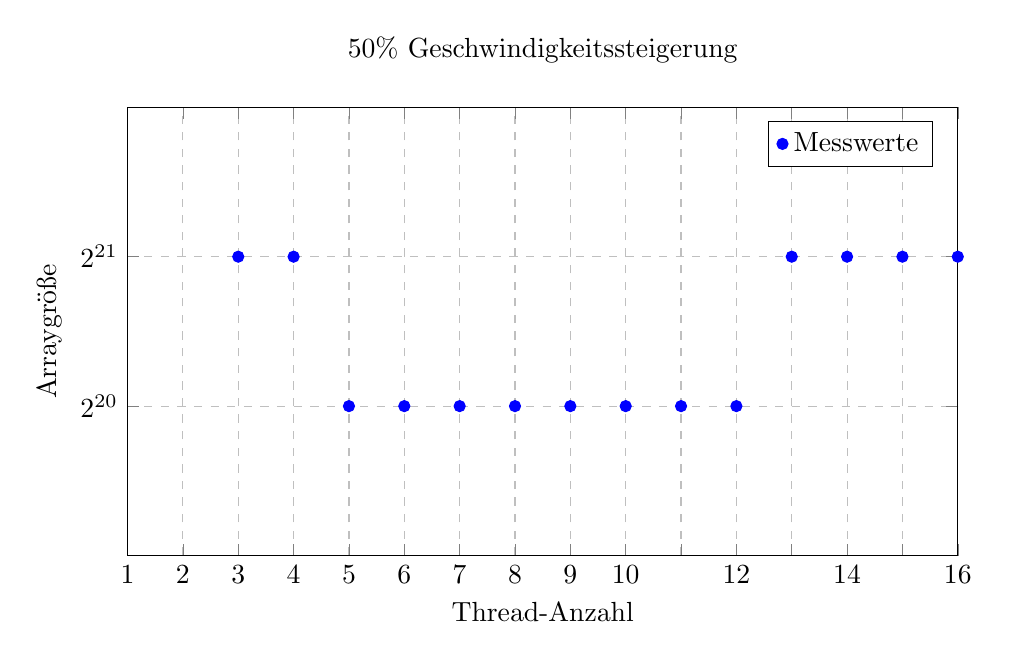
\begin{tikzpicture}
        \begin{axis}[
                title style={yshift=1.5ex},
                width=1\textwidth,
                height=0.6\textwidth,
                xlabel={Thread-Anzahl},
                ylabel={Arraygröße},
                title={50\% Geschwindigkeitssteigerung}, % Zeitpunkt der 50\% Geschwindigkeitssteigerung (incAray)
                xmin=1, xmax=16,
                ymin=2^19, ymax=2^22,
                grid style=dashed,
                legend pos=north east,
                ymode=log,
                log basis y=2,
                xtick={1,...,16},               % jeden Integer von 2 bis 17
                ytick={2^20,2^21},      % gewünschte y-Werte
                xticklabels={$1$,$2$,$3$,$4$,$5$,$6$,$7$,$8$,$9$,$10$,$ $,$12$,$ $,$14$,$ $,$16$},
                grid=both,
                grid style=dashed,
            ]
            \addplot[only marks, blue, mark=*] coordinates {
                    (1,2)
                    (3,2097152)
                    (4,2097152)
                    (5,1048576)
                    (6,1048576)
                    (7,1048576)
                    (8,1048576)
                    (9,1048576)
                    (10,1048576)
                    (11,1048576)
                    (12,1048576)
                    (13,2097152)
                    (14,2097152)
                    (15,2097152)
                    (16,2097152)
                };
            \addlegendentry{Messwerte}
        \end{axis}
    \end{tikzpicture}%
}

\newcommand{\InkrementArrayDiagrammB}{%
    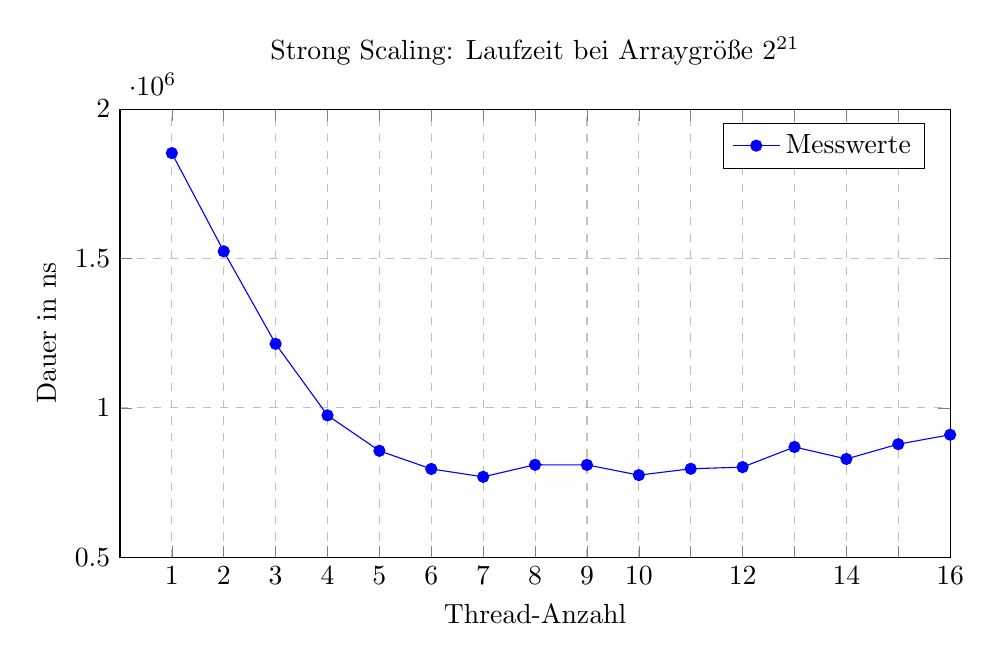
\begin{tikzpicture}
        \begin{axis}[
                title style={yshift=1.5ex},
                width=1\textwidth,
                height=0.6\textwidth,
                xlabel={Thread-Anzahl},
                ylabel={Dauer in ns},
                title={Strong Scaling: Laufzeit bei Arraygröße $2^{21}$},
                xmin=0, xmax=16,
                ymin=0.5*10^6, ymax=2*10^6,
                grid style=dashed,
                legend pos=north east,
                xtick={1,...,16},
                xticklabels={$1$,$2$,$3$,$4$,$5$,$6$,$7$,$8$,$9$,$10$,$ $,$12$,$ $,$14$,$ $,$16$},
                grid=both,
                grid style=dashed,
            ]
            \addplot[blue, mark=*] coordinates {
                    (1,1852600)
                    (2,1524000)
                    (3,1214400)
                    (4,975200)
                    (5,856500)
                    (6,795800)
                    (7,769500)
                    (8,809800)
                    (9,809400)
                    (10,775200)
                    (11,796400)
                    (12,802000)
                    (13,869400)
                    (14,829300)
                    (15,878800)
                    (16,910300)
                };
            \addlegendentry{Messwerte}
        \end{axis}
    \end{tikzpicture}%
}

\newcommand{\InkrementArrayDiagrammC}{%
    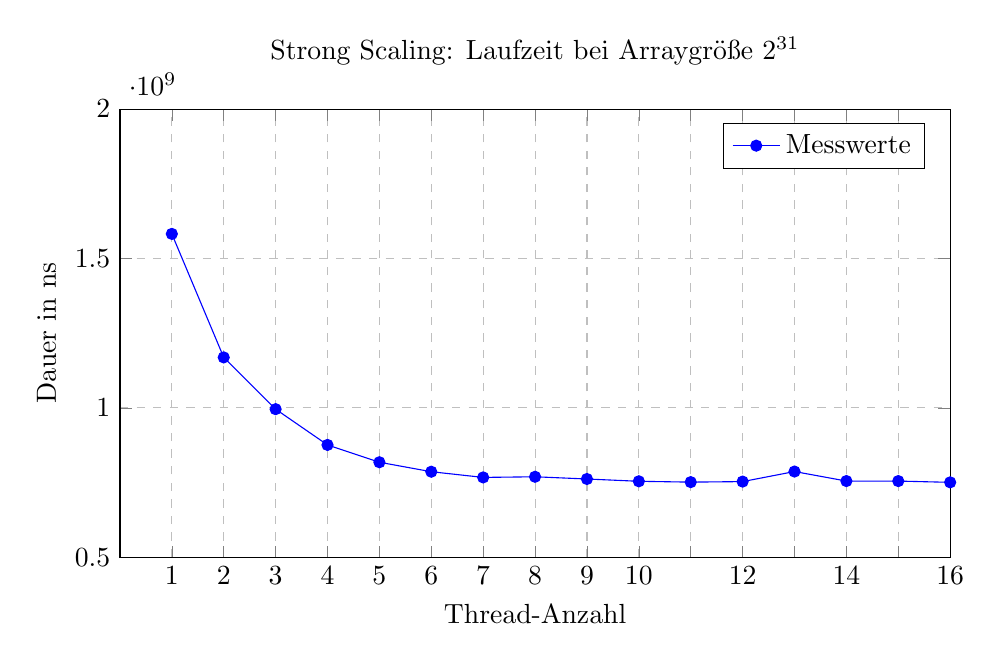
\begin{tikzpicture}
        \begin{axis}[
                title style={yshift=1.5ex},
                width=1\textwidth,
                height=0.6\textwidth,
                xlabel={Thread-Anzahl},
                ylabel={Dauer in ns},
                title={Strong Scaling: Laufzeit bei Arraygröße $2^{31}$}, % ($2^{31}-1$)
                xmin=0, xmax=16,
                ymin=0.5*10^9, ymax=0.2*10^10,
                grid style=dashed,
                legend pos=north east,
                xtick={1,...,16},
                xticklabels={$1$,$2$,$3$,$4$,$5$,$6$,$7$,$8$,$9$,$10$,$ $,$12$,$ $,$14$,$ $,$16$},
                grid=both,
                grid style=dashed,
            ]
            \addplot[blue, mark=*] coordinates {
                    (1,1582322800)
                    (2,1169109200)
                    (3,995920200)
                    (4,876230000)
                    (5,818310300)
                    (6,786585300)
                    (7,767543800)
                    (8,769668500)
                    (9,762244800)
                    (10,754572500)
                    (11,751793100)
                    (12,753548100)
                    (13,787192000)
                    (14,755368000)
                    (15,755257400)
                    (16,751066600)
                };
            \addlegendentry{Messwerte}
        \end{axis}
    \end{tikzpicture}%
}

\newcommand{\InkrementArrayDiagrammD}{%
    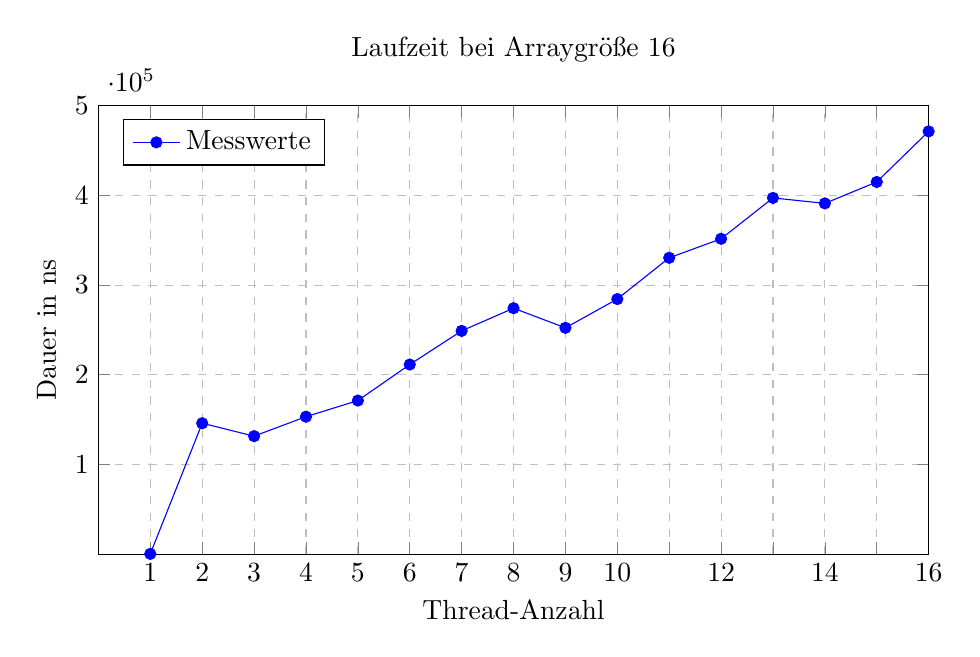
\begin{tikzpicture}
        \begin{axis}[
                title style={yshift=1.5ex},
                width=1\textwidth,
                height=0.6\textwidth,
                xlabel={Thread-Anzahl},
                ylabel={Dauer in ns},
                title={Laufzeit bei Arraygröße 16},
                grid=both,
                grid style=dashed,
                xmin=0, xmax=16,
                ymin=0, ymax=5*10^5,
                legend pos=north west,
                xtick={1,...,16},
                ytick={1*10^5,2*10^5,3*10^5,4*10^5,5*10^5},
                xticklabels={$1$,$2$,$3$,$4$,$5$,$6$,$7$,$8$,$9$,$10$,$ $,$12$,$ $,$14$,$ $,$16$},
            ]
            \addplot[blue, mark=*] coordinates {
                    (1,200)
                    (2,145900)
                    (3,131500)
                    (4,153200)
                    (5,171200)
                    (6,211400)
                    (7,248900)
                    (8,274200)
                    (9,252300)
                    (10,284400)
                    (11,330400)
                    (12,351600)
                    (13,397200)
                    (14,391100)
                    (15,415000)
                    (16,471400)
                };
            \addlegendentry{Messwerte}
        \end{axis}
    \end{tikzpicture}%
}

\newcommand{\InkrementArrayDiagrammE}{%
    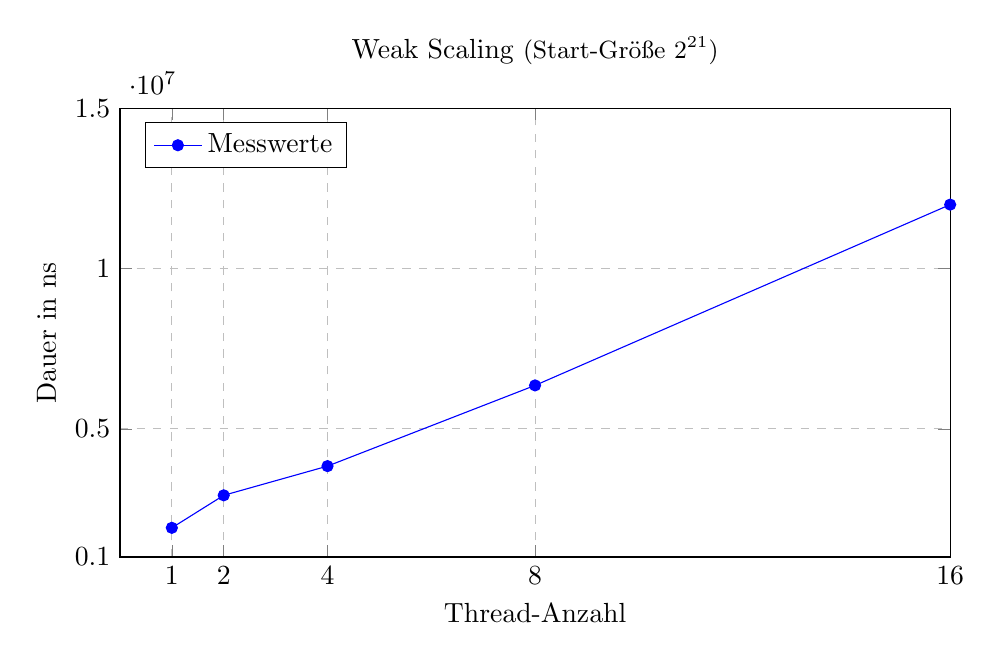
\begin{tikzpicture}
        \begin{axis}[
                title style={yshift=1.5ex},
                width=1\textwidth,
                height=0.6\textwidth,
                xlabel={Thread-Anzahl},
                ylabel={Dauer in ns},
                title={Weak Scaling {\small (Start-Größe $2^{21}$)}}, % Threads und Länge verdoppeln
                xmin=0, xmax=16,
                ymin=1*10^6, ymax=1.5*10^7,
                grid style=dashed,
                legend pos=north west,
                xtick={1,2,4,8,16},
                ytick={1*10^6, 5*10^6, 10*10^6, 1.5*10^7},
                grid=both,
                grid style=dashed,
            ]
            \addplot[blue, mark=*] coordinates {
                    (1,1910700)
                    (2,2925400)
                    (4,3837500)
                    (8,6358100)
                    (16,12003500)
                };
            \addlegendentry{Messwerte}
        \end{axis}
    \end{tikzpicture}%
}

\newcommand{\InkrementArrayDiagrammF}{%
    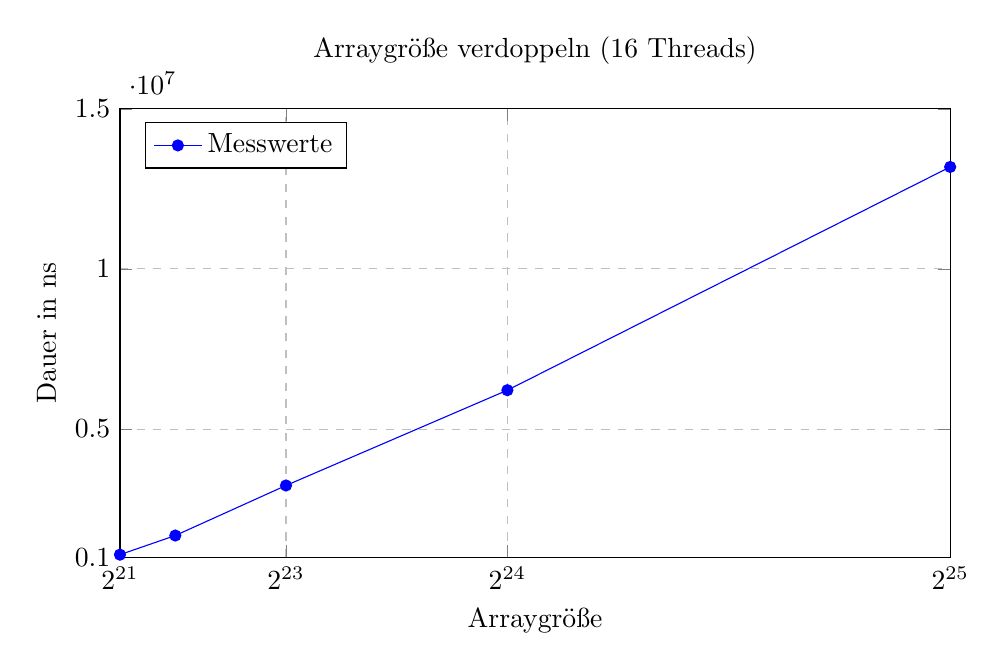
\begin{tikzpicture}
        \begin{axis}[
                title style={yshift=1.5ex},
                width=1\textwidth,
                height=0.6\textwidth,
                xlabel={Arraygröße},
                ylabel={Dauer in ns},
                title={Arraygröße verdoppeln (16 Threads)},
                xmin=2^21, xmax=1 * 2^25,
                ymin=1*10^6, ymax=1.5*10^7,
                grid style=dashed,
                legend pos=north west,
                xtick={2^21,2^23,2^24,2^25},
                xticklabels={$2^{21}$, $2^{23}$, $2^{24}$, $2^{25}$},
                scaled x ticks=false,
                ytick={1*10^6, 5*10^6, 10*10^6, 1.5*10^7},
                grid=both,
                grid style=dashed,
            ]
            \addplot[blue, mark=*] coordinates {
                    (2097152,1077100)
                    (4194304,1675200)
                    (8388608,3237700)
                    (16777216,6213600)
                    (33554432,13184900)
                };
            \addlegendentry{Messwerte}
        \end{axis}
    \end{tikzpicture}%
}

\newcommand{\InkrementArrayText}{
    Anhand dieses einfachen Beispiels soll gezeigt werden, was Parallelisierung in der Praxis bewirkt und dass die Praxis nicht immer mit den Erwartungen übereinstimmt. Zudem stellt dieses Beispiel einen guten Einstieg in das Thema Parallelisierung dar.
    An den Diagrammen (Abbildung~\ref{fig:InkrementArrayDiagramm}) ist deutlich zu erkennen, dass dieses Beispiel nicht linear mit der Thread-Anzahl skaliert, obwohl dies rein theoretisch zu erwarten wäre. Dies liegt wahrscheinlich an der Speicherlatenz als limitierendem Faktor. Dies würde erklären, warum ab einem gewissen Punkt mehr ausgelastete Kerne keinen weiteren Performancegewinn mehr bringen. Zudem ist zu erkennen, dass das Array mindestens $2^{20}$ groß sein muss, damit eine parallele Ausführung einen mindestens zweifachen Geschwindigkeitsvorteil gegenüber der sequenziellen Laufzeit erreicht.
    Zusätzlich ist anzumerken, dass die sequenzielle Laufzeit dieser Funktion normalerweise unter 100~ns liegt. Dies ist auf Compiler-Optimierungen zurückzuführen. Daher wurde diese Funktion mit \texttt{volatile} ausgeführt, was verhindert, dass der Compiler die eigentliche Aufgabe herausoptimiert und sie somit messbar bleibt. Das \texttt{volatile}-Schlüsselwort sorgt dafür, dass bei jedem Lesevorgang die Daten aus dem RAM geladen werden müssen. Daher ist es auch das wahrscheinlichste Szenario, dass dieses Beispiel durch das Datenratenlimit begrenzt ist. Zusätzlich ist die eigentliche Aufgabe trivial für die CPU und lastet diese daher nicht vollständig aus.
    Aufgrund dieses künstlich erzeugten Szenarios durch die bewusste Beeinflussung des Laufzeitverhaltens mit \texttt{volatile} wird auf eine detaillierte Einzelanalyse der Diagramme verzichtet.
}



\newcommand{\InkrementArray}{
    % Inkrement-Array
    \InkrementArrayText
    \newline
    %\resizebox{\textwidth}{8cm}{%
    \begin{minipage}{\textwidth}
        \centering
        % Zeile 1
        \begin{minipage}{0.48\textwidth}
            \centering \InkrementArrayDiagrammA
            \captionof{figure}[Inkrement-Array (50\% Geschwindigkeitssteigerung)]{
                Zeigt, ab welcher Arraygröße zum ersten Mal eine 50\,\% höhere Geschwindigkeit als die sequentielle Laufzeit erreicht wird.
            }
        \end{minipage}\hfill %
        \begin{minipage}{0.48\textwidth}
            \centering \InkrementArrayDiagrammD
            \captionof{figure}[Inkrement-Array (Laufzeit bei Arraygröße 16)]{
                Zeigt die Overheads, die durch Threads entstehen.
            }
        \end{minipage}
        \par\vspace{1em}

        % Zeile 2
        \begin{minipage}{0.5\textwidth}
            \centering \InkrementArrayDiagrammB
            \captionof{figure}[Inkrement-Array (Laufzeit bei Arraygröße $2^{21}$)]{}
        \end{minipage}%
        \begin{minipage}{0.5\textwidth}
            \centering \InkrementArrayDiagrammC
            \captionof{figure}[Inkrement-Array (Laufzeit bei Arraygröße $2^{31}$)]{}
        \end{minipage}
        \par\vspace{1em}

        % Zeile 3
        \begin{minipage}{0.5\textwidth}
            \centering \InkrementArrayDiagrammE
            \captionof{figure}[Inkrement-Array (Weak Scaling {\small (Start-Größe $2^{21}$)})]{}
        \end{minipage}%
        \begin{minipage}{0.5\textwidth}
            \centering \InkrementArrayDiagrammF
            \captionof{figure}[Inkrement-Array (Arraygröße verdoppeln (16 Threads))]{}
        \end{minipage}

        \captionof{figure}[Laufzeitanalyse Inkrement-Array]{Laufzeitanalyse Inkrement-Array}
        \label{fig:InkrementArrayDiagramm}
    \end{minipage}
    %}
}